\begin{figure}
\centering

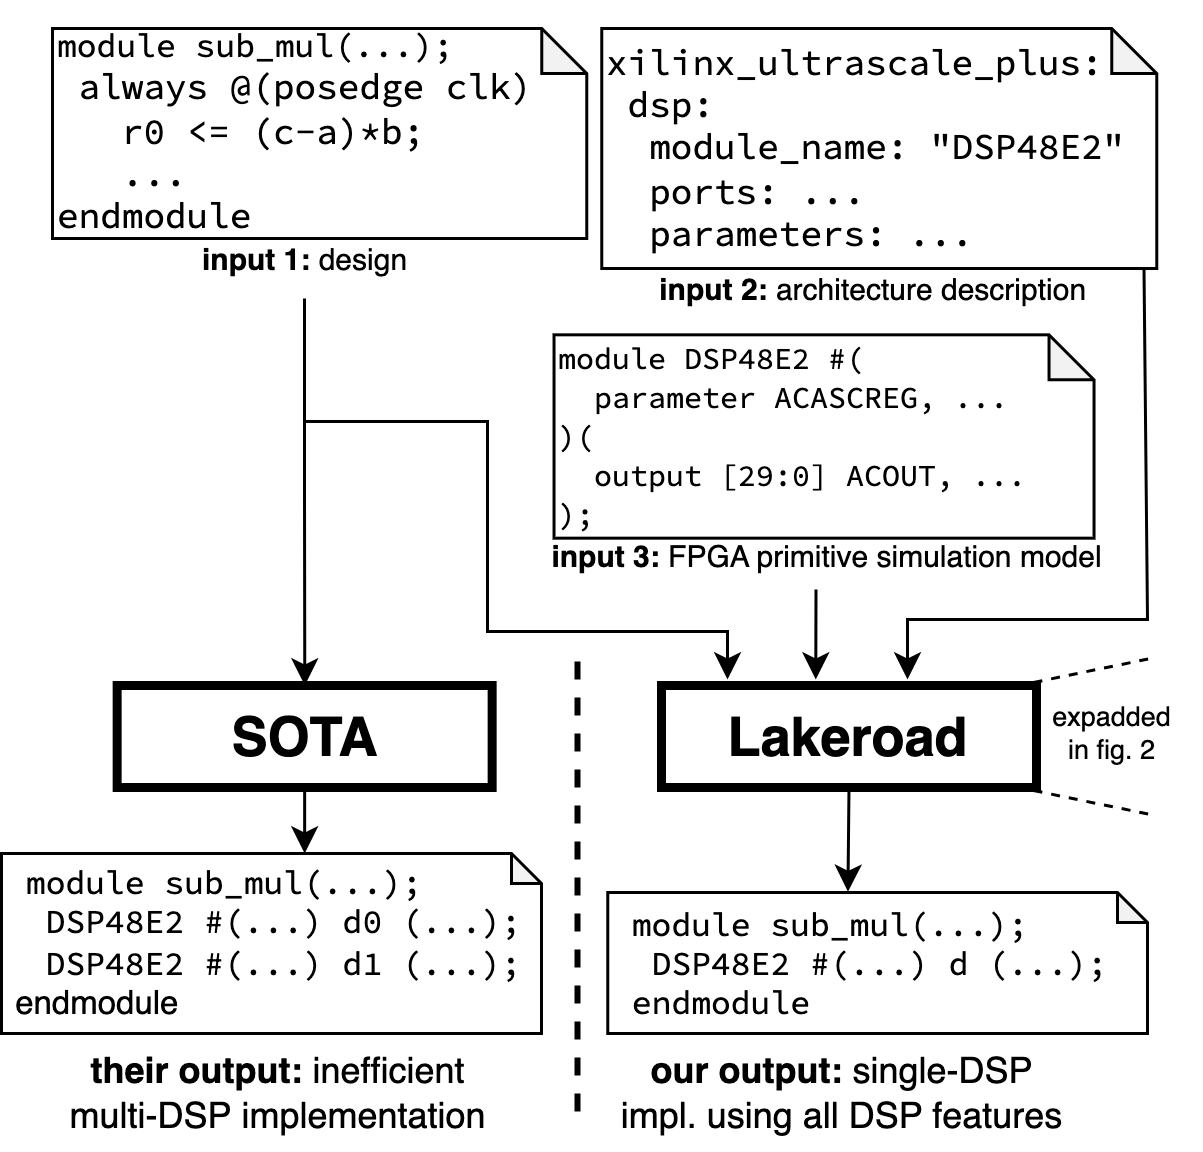
\includegraphics[width=0.91\columnwidth]{assets/lakeroad-firstpage.drawio.png}

% \vspace{3mm}
% \resizebox{0.4\textwidth}{!}{
% \begin{tabular}{cc|c|c}
% Design& \# Stages &  SOTA& \lr \\ \hline
% \texttt{((d+a)*b)|c}& 1 &2 DSP, 18 LUT & 1 DSP  \\
% \texttt{((d+a)*b)\textasciicircum{}c} & 1 & 2 DSP, 18 LUT  & 1 DSP \\
% \texttt{((d-a)*b)|c} & 2 & 2 DSP, 18 LUT & 1 DSP \\
% \texttt{((d-a)*b)\textasciicircum{}c} &  2          & 2 DSP, 18 LUT & 1 DSP \\
% \texttt{((d+a)*b)\&c}& 2 & 2 DSP, 18 LUT & 1 DSP \\
% \end{tabular}}
\vspace{-3mm}
\caption{
% Mapping a simple design to
%   Xilinx UltraScale+ FPGAs with both
%   the state of the art (SOTA)
%   hardware synthesis tool for Xilinx
%   and \lr.
Even given a simple input
  design (input 1),
  the state-of-the-art (SOTA)
  hardware synthesis tool
  for Xilinx FPGAs
  frequently
  fails to efficiently use 
  programmable primitives
  like DSPs.
\lr,
  on the other hand,
  can utilize all features
  of programmable primitives
  given just a short description
  of an FPGA architecture (input 2)
  and the vendor-provided 
  simulation models
  of the primitive (input 3).\tighten
}
\label{fig:firstpage}

\vspace{-5mm}
\end{figure}


\textit{\Cref{part:lakeroad} is adapted from 
``FPGA Technology Mapping Using Sketch-Guided Program Synthesis'' by Smith, et al.~\cite{smith2024fpga}.
}

\vspace{10mm}

\noindent
Given a high-level hardware design specification
  (e.g., expressed in behavioral Verilog),
  FPGA technology mappers
  search for an equivalent
  low-level implementation
  in terms of the target FPGA's
  primitives.
See \cref{fig:firstpage} for an example, where
the high-level, behavioral \texttt{sub\_mul}
  module (``input 1'')
  is converted into FPGA-specific implementations
  (``their output'' and ``our output'')
  using the Xilinx-specific
  \texttt{DSP48E2} primitive.
  
Historically,
  FPGAs consisted of relatively simple
  primitives, such as
  lookup tables (LUTs) and carry chains.
Tools like
  ABC~\cite{ABC,abc2,brayton2010abc}
  \textit{automatically} 
  map to these basic primitives
  by translating designs
  to a library of simple logic gates
  and then packing those gates
  into LUTs.

However, FPGAs are becoming
  increasingly heterogeneous
  via
  the inclusion of specialized and diverse primitives
  such as digital signal processors (DSPs).
Utilizing these specialized primitives
  effectively
  is now
  crucial for achieving
  high performance~\cite{vega2021reticle}.
  % possibly relevant cite: zhu2022fpgaheterogeneity
These specialized primitives
  make FPGA technology mapping far more challenging
  since technology mappers must now
  explore a much larger search space
  while also satisfying each primitive's
  complex set of restrictions and dependencies.
% Despite the growing importance of effective technology mapping,
%   these specialized primitives
% make it far more challenging since technology mappers must now
%   explore a much larger search space
%   while also satisfying each primitive's
%   complex set of restrictions and dependencies.
For example, Xilinx's DSP48E2
  is a multifunction 
  DSP
  with nearly
  100 ports and parameters,
  whose numerous configurations
  enable 
  support for a large variety of computations.
The manual for the DSP48E2 alone
  is 75 pages long,
  where considerable text details
  the complex restrictions
  between the settings of the nearly 100
  ports and parameters.

Existing technology mapping tools
  frequently fail to map designs
  to
  specialized primitives like DSPs,
  resulting in less-performant designs
  (that is, poor \cref{thesis:optimizations})
  and
  requiring manual work for the hardware designer
  to recover the performance of their design
  (that is, increased \cref{thesis:devtime}).
While existing toolchains
  have the ability to automatically infer
  locations where specialized primitives
  can be used in large designs,
  inference often fails~\cite{xilinxforum1,xilinxforum2,inferringreddit}.
In these cases, the designer can either
  accept lower performance and higher resource
  utilization,
  or they can perform
  what we call
  \textit{partial design mapping.}
During partial design mapping, 
  the designer
  manually identifies and separates out
  the module that should be mapped
  to a DSP.
They can attempt to re-run technology mapping
  on that module alone,
  in the hopes that mapping succeeds.
Yet existing toolchains often fail
  \textit{even in the partial design mapping case:}
  \cref{fig:firstpage} shows a
  simple module
  \texttt{sub\_mul}
  which \textit{should} fit on a single DSP48E2
  according to the DSP's manual,
  but is instead mapped to 
  two DSPs by current 
  state-of-the-art tools\footnote{
    Licensing restrictions forbid naming the
    specific proprietary tools, but they are familiar,
    standard packages used by many hardware designers.
  }---%
  a 100\% increase in resource utilization!
In the worst case,
  hardware designers are forced to manually
  instantiate complex primitives by hand,
  e.g., by looking through the 75-page
  DSP48E2 user manual
  to manually configure the DSP's dozens
  of ports and parameters.

Current state-of-the-art
  technology mappers 
  are implemented via
  ad hoc, handwritten pattern matching procedures,
  which
  fall short in three primary ways.
First,
  as we saw above,
  they are \textbf{incomplete:}
  they miss many mapping opportunities,
  even across microbenchmarks based on vendor documentation
  (\cref{thesis:optimizations}).
Second, they do not provide strong \cref{thesis:correctness} guarantees:
  recent work highlights the significant number of bugs found across 
  all major hardware synthesis tools~\cite{herklotz2020finding}.
Third, they are difficult to extend:
  \textit{each} new complex primitive requires
  supporting detailed semantics
  and adding hundreds of new, special-case
  syntactic pattern matching rules~\cite{wolf2013yosys}
  (hence increasing \cref{thesis:devtime}).


This chapter's
  key observation is that 
  technology mapping
  is well-suited for the application
  of automated reasoning procedures
  (\cref{thesis:algorithms})---%
  specifically,
  \textit{program synthesis}~\cite{gulwani2017program}.
We observe that 
  the configuration space of
  a programmable FPGA primitive
  is essentially a small, bespoke
  programming language,
  and that
  program synthesis
  could be applied
  to automatically generate
  primitive configurations.
  % that is used
  % to map design fragments
  % down to those low-level 
  % primitives.
% \asplos{Our second observation
%   is that,
%   though the number of possible 
%   configurations
%   for each specialized primitive
%   is large,
%   the problem size is
%   well within
%   the bounds for computer-aided
%   reasoning techniques.}
We explore how
  program synthesis
  can simplify the design and implementation of
  FPGA technology mappers while providing
  \textbf{correct} (\cref{thesis:correctness}),
  \textbf{extensible} (\cref{thesis:devtime}), and
  \textbf{more complete}
  (\cref{thesis:optimizations})
  support for mapping to 
  diverse, highly configurable primitives
  like DSPs.
Program synthesis techniques rely on
  automated theorem provers like
  SAT and SMT solvers~\cite{de2008z3, barbosa2022cvc5}
  to automatically generate programs
  satisfying a given specification.
We demonstrate how
 \textit{sketch-guided program synthesis}~\cite{solar2008program}
  can be adapted
  for FPGA technology mapping,
  leveraging the
  Rosette~\cite{torlak2014lightweight} 
  program synthesis framework.
% The below seems like WAY too much detail for the intro. It also feels like it's out of place in this paragraph.
%   given a specification as a
%   design fragment $D$ expressed in behavioral HDL,
%   we use the Rosette~\cite{torlak2014lightweight} program synthesis framework embedded in the Racket language
%   to efficiently search for
%   configurations of
%   low-level, FPGA-specific primitives,
%   i.e., programs in structural HDL
%   that implement $D$.\tighten

% We developed two new techniques to enable
%   building correct, extensible, and more-complete
%   FPGA technology mappers
%   via program synthesis:
%   (1) \textbf{semantics extraction from HDL}
%       to provide mostly-automated encoding of the
%       programming language and semantics
%       for each kind of FPGA primitive, and
%   (2) \textbf{architecture-independent sketch templates}
%       to encode generic, high-level implementation strategies
%       that efficiently map design fragments across
%       multiple FPGA architectures.

Sketch-guided program synthesis requires
  encoding the \textit{semantics}
  of the target language:
  in our case,
  a machine-readable,
  mathematical model specifying
  the behavior of each
  FPGA-specific primitive
  being mapped to.
In a typical synthesis tool,
  which generates programs
  for a single target language,
  this is a one-time cost.
However,
  in our setting,
  each new FPGA primitive
  introduces yet another new target language,
  which in turn requires
  extending the tool to encode
  yet another formal semantics.

To support
  correct, extensible, and more complete
  technology mapping, we propose
  automating this process with
  \textbf{semantics extraction from HDL}, 
  adapted from past work~\cite{daly2022synthesizing},
  to automatically extract
  complete primitive semantics
  from vendor-published HDL 
  \cref{thesis:models}
  (\cref{fig:firstpage}, ``input 3'').
Traditionally, such models have
   been used only 
  for
  simulation and validation
  \textit{after} technology mapping;
  we show that using the semantics
  to
  \textit{implement}
  technology mapping
  with a program-synthesis-based approach
  yields substantially more
  complete FPGA technology mapping.

Sketch-guided program synthesis also
  requires \textit{sketches}, which are 
  partially complete programs with ``holes'' to be filled in
  by the solver.
Sketches primarily serve to
  scale synthesis by
  constraining the set of programs that 
  solvers explore when searching for
  one that satisfies
  the given specification,
  i.e., performance at the cost of completeness.
In our setting,
  sketches correspond to
  arrangements of primitives,
  using holes
  as placeholders
  for some of the primitives' 
  ports and parameters.
This could be
  a single DSP with holes for
  its ports and parameters
  (as in the example in \cref{sec:overview-part-2}),
  or a number of LUTs with holes for their LUT memories,
  or even a mixture of LUTs, DSPs, and carry chains.
The synthesizer ``fills in the holes''
  as necessary for
  the low-level FPGA-specific primitive to implement
  a given high-level behavioral design fragment.
Unfortunately,
  developing effective sketches
  still requires synthesis expertise~\cite{10.1145/3140587.3062353,vanGeffenJITSynth}.
  Na\"ively, our approach would also
  require new sketches for each new
  FPGA primitive we target.


% %Naively, both obtaining
%   %semantics and
%   %writing sketches would
%   %hamper a program synthesis
%   %approach to technology mapping.
% At first glance,
%   obtaining semantics
%   and writing sketches
%   would appear to be difficult
%   manual steps
%   that would impede the use of program synthesis
%   and negating any benefits of automation.
% (Incidentally, current
%   technology mappers also manually
%   specify the semantics
%   via 
%   their unstructured hand-written 
%   patterns and procedures.)
% % Current technology mappers only
% %   reason about primitive semantics
% %   in the unstructured hand-written 
% %   procedures,
% %   and requiring users
% %   to provide sketches
% %   would hamper extensibility, 
% %   as sketches require primitive-specific details
% %   that would negate the automation benefit
% %   of such an approach. 
% However, we apply two key insights
%   to make this approach practical.

 
To address these challenges, 
  we introduce
  \textbf{architecture-independent sketch templates.}
% There are a few common classes 
%   of
%   FPGA primitives
%   present across most architectures:
%   LUTs, carry chains, muxes, and DSPs.
Hardware designs are often implemented
  using high-level blueprints that are similar 
  across most FPGA architectures---%
  sketch templates
  capture these blueprints
  and make them reusable across architectures.
Therefore, by using sketch templates, we
  greatly reduce the overhead of supporting
  new architectures and
  diverse primitives.
Typically, when adding support for
  a new primitive or FPGA architecture in \lr,
  the hardware designer
  need not write or modify
  any sketch templates.


% However,
%   FPGA primitives across architectures
%   fall into a few common classes, e.g.,
%   LUTs, carry chains, and DSPs, and
%   the way these primitives
%   are used to implement designs
%   is similar across architectures.
% Hence, we introduce abstractions
%   to capture these similarities to build
%   \textbf{architecture-independent
%   sketch templates},
%   reducing the effort required to
%   support a new primitive.



We leverage
  semantics extraction
  from HDL
  and architecture-independent
  sketch templates
  to build \lr,\footnote{
  \lr is publicly available at
  \url{https://github.com/uwsampl/lakeroad}.
  }
  a new FPGA technology mapper
  based on program synthesis.
  
\lr's prototype implementation automatically
  imports semantics for the LUTs, arithmetic carry chains,
  and DSPs of the Xilinx UltraScale+, Lattice ECP5,
  Intel Cyclone 10 LP,
  and SOFA~\cite{sofa} FPGA architectures. 
The only additional user input to \lr is a short 
  architecture description
  that lists the target FPGA's
  primitives (\cref{fig:firstpage}, ``input 2'').
Architecture descriptions
  only need to be written once per architecture,
  and \lr pre-supplies architecture descriptions
  for the aforementioned architectures.
With the automatically
  extracted primitive semantics
  and the user-provided architecture description,
  we demonstrate that \lr
  is more complete than proprietary tools on a variety
  of microbenchmarks
that are representative of program fragments
  implemented with DSPs during partial design mapping.
In particular,
  \lr maps up to 3.6$\times$ 
  more microbenchmarks than 
  state-of-the-art
  tools for Xilinx, Lattice, and Intel,
  and up to 30$\times$ 
  more microbenchmarks 
  than Yosys.\looseness=-1
% We further show the practical applicability
%   of \lr
%   in real-world applications
%   by integrating it into the open-source
%   hardware synthesis tool
%   Yosys~\cite{wolf2013yosys}.
%\sandy{Note that this is a long list of contributions, which "usually" (in most papers I read) number a more memorable 3 or 4. Can any contributions be combined for ease or reader retention? }

\Cref{part:lakeroad} of this dissertation
makes
  the following key contributions:
\begin{itemize}[leftmargin=*]
\item The novel application of program synthesis
  to produce a technology mapper---\lr---that is
  more \textbf{correct, complete,} and \textbf{extensible} than state-of-the-art 
  tools.
\item A technique for applying
  \textbf{semantics extraction from HDL}
  to automatically generate models
  of hardware usable by 
  formal automated reasoning tools.
\item The concept of 
  \textbf{architecture-independent sketch templates,}
  which capture common patterns in hardware design
  in an architecture-independent way,
  plus \textbf{primitive interfaces} and \textbf{architecture descriptions}, the abstractions
  underlying these templates.
  % \begin{itemize}
  %     \item \textbf{Primitive interfaces,} 
  %       which abstract common primitives across FPGA architectures.
  %     \item \textbf{Architecture descriptions,}
  %       a text format for specifying how primitive interfaces
  %       are implemented
  %       on a specific FPGA architecture.
  % \end{itemize}
% \item \textbf{\lrir, a domain-specific language (DSL)}
%   that captures hardware design sketches.
% \item Formal semantics
%   languages for combinational and sequential logic, 
\item A formalization of the \lr
  toolchain and an argument
  for its correctness and sketch-completeness.
\item The first notion of \textbf{technology
  mapping completeness} for FPGA
  compilers.
\item \textbf{Empirical comparisons }of
  \lr and existing hardware synthesis
  tools to evaluate both their
  relative completeness and
  ease of extensibility.


  
% \item The \lr prototype toolchain for
%   practical FPGA technology mapping 
%   via program synthesis.


% \item An evaluation of \lr mapping
%     primitives on Xilinx, Lattice, Intel,
%     and SOFA
%     FPGAs.

\end{itemize}

In the following sections, we walk through a real-world example
  using both existing tools
  and \lr
  and 
  highlight \lr's design and key features (\cref{sec:overview}); 
  formalize \lr and
  demonstrate its correctness (\cref{sec:formalization}); 
  describe \lr's implementation (\cref{sec:implementation}); and 
  evaluate \lr on its
  completeness of mapping,
  extensibility,
  and expressiveness (\cref{sec:evaluation}) .
  % terms of
  % effort to synthesize technology mappers
  % and the quality of the generated FPGA
  % implementations.
\cref{sec:background-and-related-work}
  discusses related work, and
  \cref{sec:lakeroad-conclusion} concludes.